\section{Results}
% \begin{frame}[c]{Results on Object Classification}
%     \todo{Picture of input/output}
% \end{frame}
\begin{frame}[c]{Results on Object Classification}
    \begin{columns}
        \centering
        \column{0.7\textwidth}
        \begin{table}[!ht]
    % 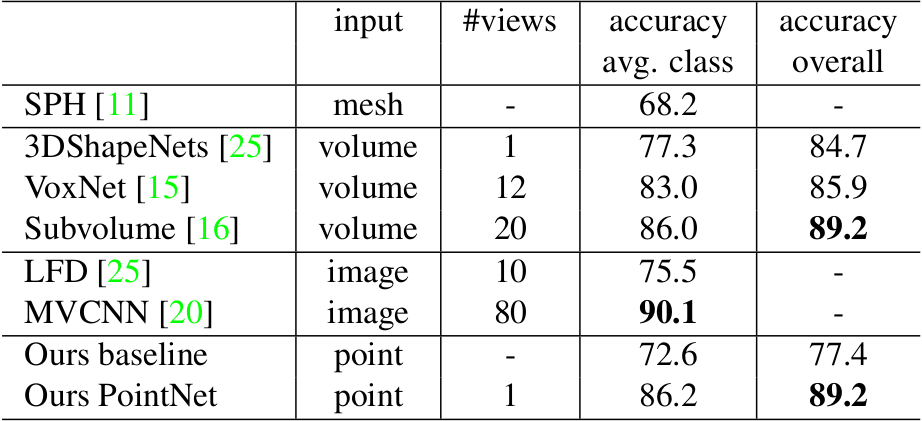
\includegraphics[width=0.5\textwidth]{modelnet}
    \normalsize
    \begin{tabular}{l|c|c|c|c}
        & input & \#views & accuracy & accuracy \\
        & & & avg. class & overall \\ \hline
        SPH \cite{kazhdan2003rotation} & mesh & - & 68.2 & - \\ \hline

        3DShapeNets \cite{wu20153d}     & volume & 1 & 77.3 & 84.7 \\
        VoxNet \cite{maturana2015voxnet} & volume & 12 & 83.0 & 85.9 \\
        Subvolume \cite{qi2016volumetric} & volume & 20 & 86.0 & \textbf{89.2} \\ \hline

        LFD \cite{wu20153d} & image & 10 & 75.5 & - \\
        MVCNN \cite{su2015multi} & image & 80 & \textbf{90.1} & - \\ \hline

        Ours baseline & point & - & 72.6 & 77.4 \\
        Ours PointNet & point & 1 & 86.2 & \textbf{89.2} \\
    \end{tabular}
    \caption{
        \textbf{Classification results on ModelNet40.}
        PointNet achieves state-of-the-art among deep nets on 3D input.
        % Our net achieves
        % state-of-the-art among deep nets on 3D input." Table and caption taken
        % from \cite{qi2017pointnet}. \todo{rewrite in own words}
        Table from \cite{qi2017pointnet}.
    } \label{table:modelnet}
\end{table}

    \end{columns}
    \pnote{In Klassifikation wurde SOTA erreicht.}
\end{frame}


\begin{frame}[c]{Visualization of Object Part Segmentation}
    \begin{columns}
        \column{0.1\textwidth}
        \column{0.7\textwidth}
        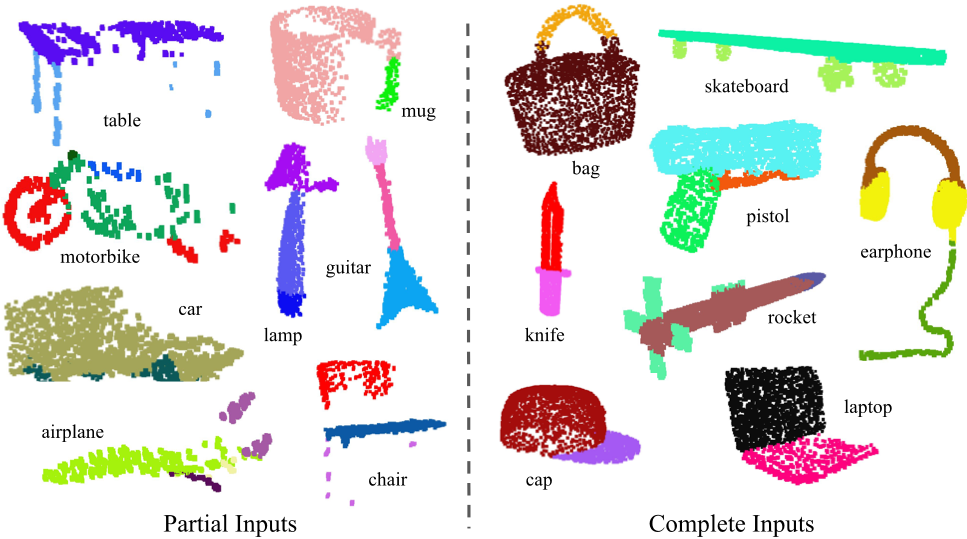
\includegraphics[height=0.75\textheight]{p46_55}
        \column{0.2\textwidth}
        \color{ocre}{Figure from \cite{qi2017pointnet}.}
    \end{columns}
    \pnote{Andere Aufgabe: Segmentieren von (partiellen) Eingaben}
\end{frame}


\begin{frame}[c]{Results on Object Part Segmentation}
    \begin{figure}
        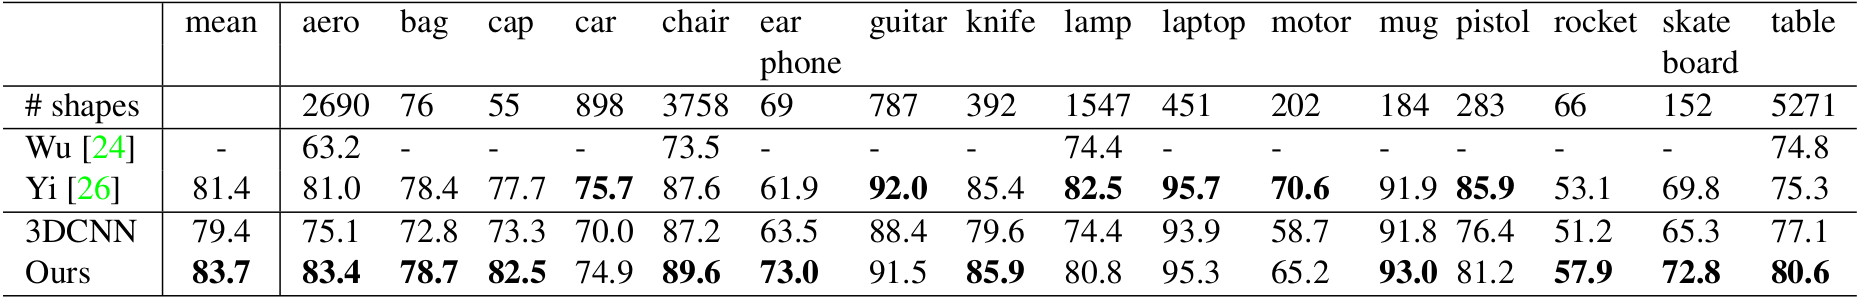
\includegraphics[width=\textwidth]{shapenet}
        \caption{
            \textbf{Segmentation results on ShapeNet part dataset.} The metric
            used is mIoU(\%) on points. Figure/Table from \cite{qi2017pointnet}.}
    \end{figure}
    \pnote{
        Hier wurde eine neue SOTA gesetzt
    }
\end{frame}

\begin{frame}[c]{Semantic Scene Parsing}
    % \begin{figure}[htb]
    \centering % <-- added
    \begin{subfigure}{0.25\textwidth}
        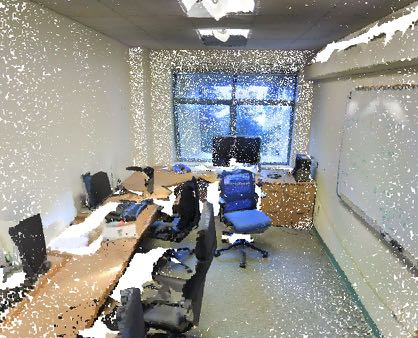
\includegraphics[width=\linewidth]{p48_58}
    \end{subfigure}\hfil % <-- added
    \begin{subfigure}{0.25\textwidth}
        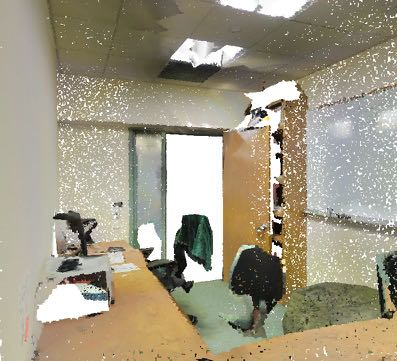
\includegraphics[width=\linewidth]{p48_59}
    \end{subfigure}\hfil % <-- added
    \begin{subfigure}{0.25\textwidth}
        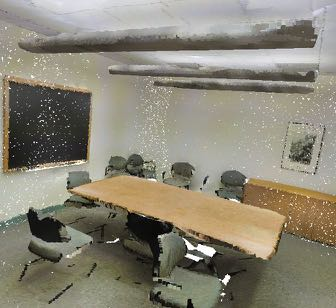
\includegraphics[width=\linewidth]{p48_61}
    \end{subfigure}

    \medskip
    \begin{subfigure}{0.25\textwidth}
        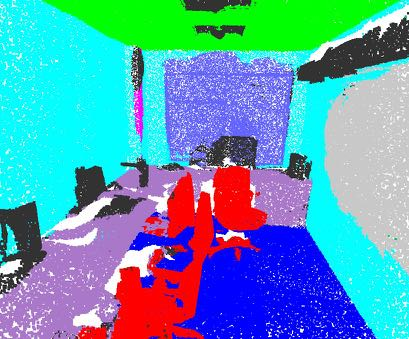
\includegraphics[width=\linewidth]{p48_57}
    \end{subfigure}\hfil % <-- added
    \begin{subfigure}{0.25\textwidth}
        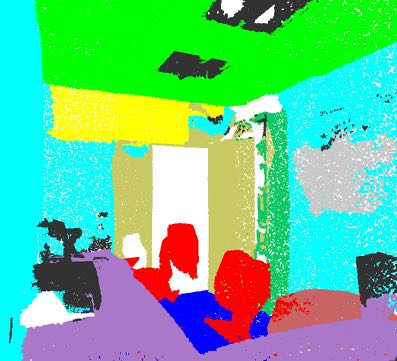
\includegraphics[width=\linewidth]{p48_60}
    \end{subfigure}\hfil % <-- added
    \begin{subfigure}{0.25\textwidth}
        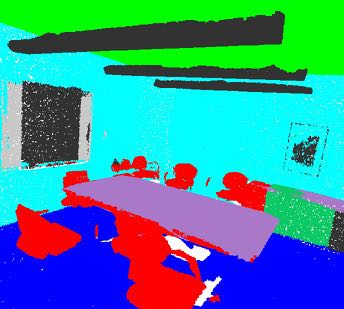
\includegraphics[width=\linewidth]{p48_62}
    \end{subfigure}
    \caption{Figures from \cite{qi2017pointnet}.}
\end{figure}


    \Large
    \begin{columns}
        \column{0.15\textwidth}
        \begin{itemize}
            \item Input
                \vspace{3em}
            \item Output
        \end{itemize}
        \column{0.2\textwidth}
        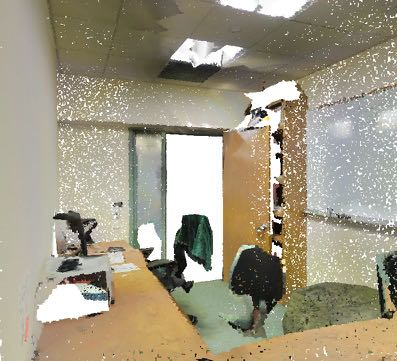
\includegraphics[width=\textwidth]{p48_59} \\
        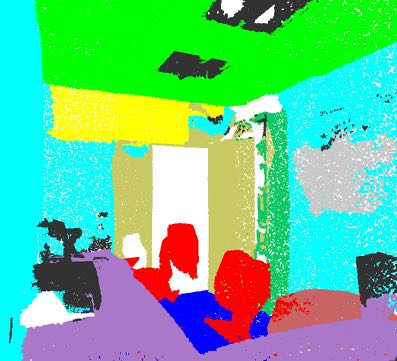
\includegraphics[width=\textwidth]{p48_60}
        \column{0.22\textwidth}
        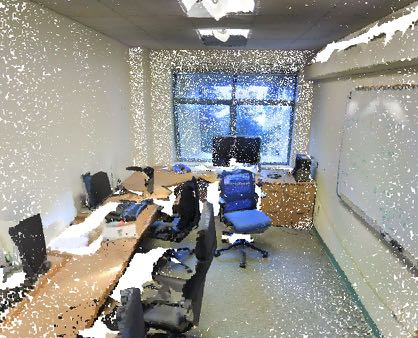
\includegraphics[width=\textwidth]{p48_58} \\
        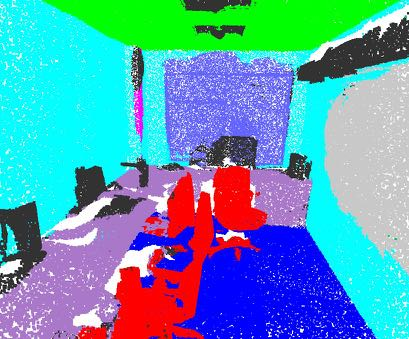
\includegraphics[width=\textwidth]{p48_57}
        \column{0.2\textwidth}
        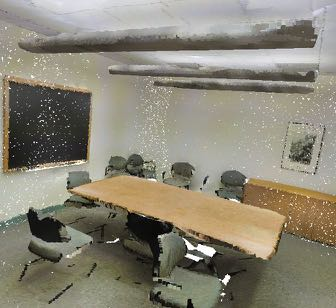
\includegraphics[width=\textwidth]{p48_61} \\
        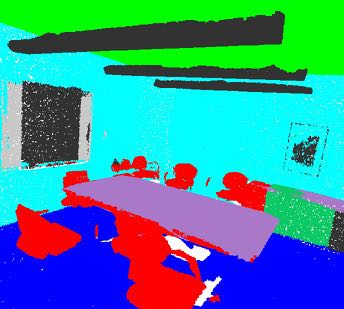
\includegraphics[width=\textwidth]{p48_62}
    \end{columns}
    \blfootnote{Figures from \cite{qi2017pointnet}.}
\end{frame}


\begin{frame}[c]{Robustness to Data Corruption}
    % \begin{figure}[!t]
    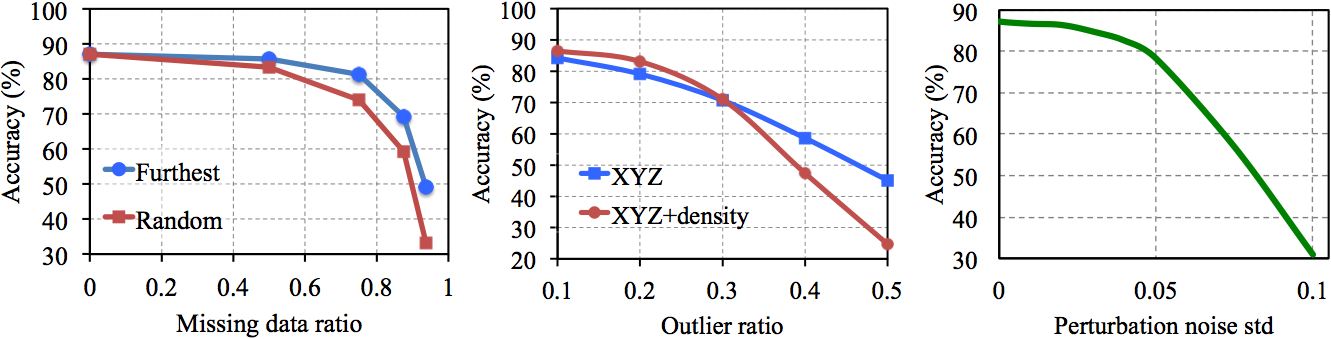
\includegraphics[width=\textwidth]{p51_65}
    \caption{
        \textbf{Robustness tests visualization.}
        Accuracy measured is overall classification accuracy on the ModelNet40
        test set. Left: Point deletion based on different sampling strategies,
        random and furthest sampling, up to the 1024 original points. Middle:
        Insertion of uniformly scattered outliers in the canonicalized unit
        sphere of the original shape. Right: Adding perturbation in the form of
        Gaussian noise with mean 0 to each point in the unit sphere independently.
        Figure from \cite{qi2017pointnet}.
        % The metric is overall classification
        % accuracy on ModelNet40 test set. Left: Delete points. Furthest means
        % the original 1024 points are sampled with furthest sampling. Middle:
        % Insertion. Outliers uniformly scattered in the unit sphere. Right:
        % Perturbation. Add Gaussian noise to each point independently." Figure
        % and caption taken from \cite{qi2017pointnet}. \todo{rewrite in own words}
    } \label{fig:robustness}
\end{figure}



    \begin{figure}
        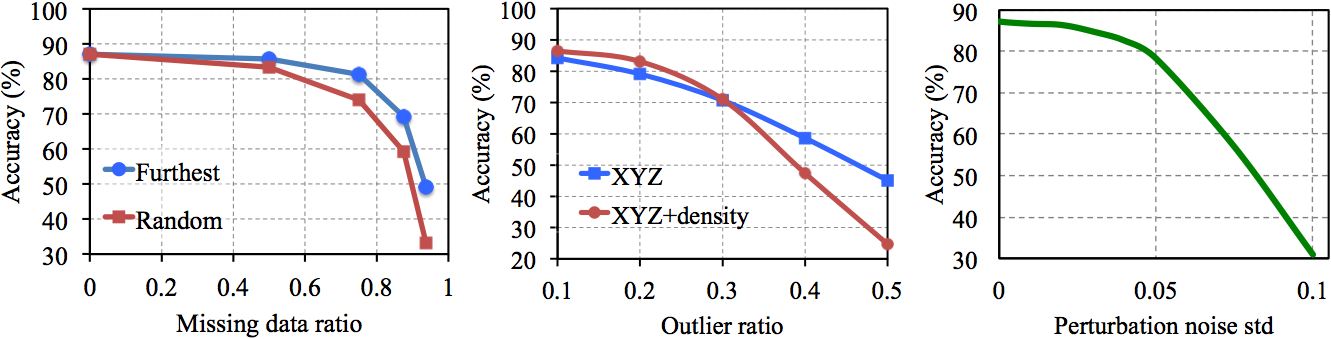
\includegraphics[width=\textwidth]{p51_65}
        \caption{
            \textbf{Robustness tests.}
            Accuracy measured on ModelNet40.
            Figure from \cite{qi2017pointnet}.
        }
    \end{figure}
    \pnote{
        Sehr Robust gegenüber dem: \\
        - Löschen von einzelnen Punkten \\
        - hinzufügen von Ausreißern \\
        - hinzufügen von extremen Rauschen \\
        \par
        Also allgemeinen störungen in Daten. \\
        Next: Anschauen woran das liegt.
    }
\end{frame}


\begin{frame}[c]{Robustness in comparison}
    \Large
    \begin{columns}
        \column{0.5\textwidth}
        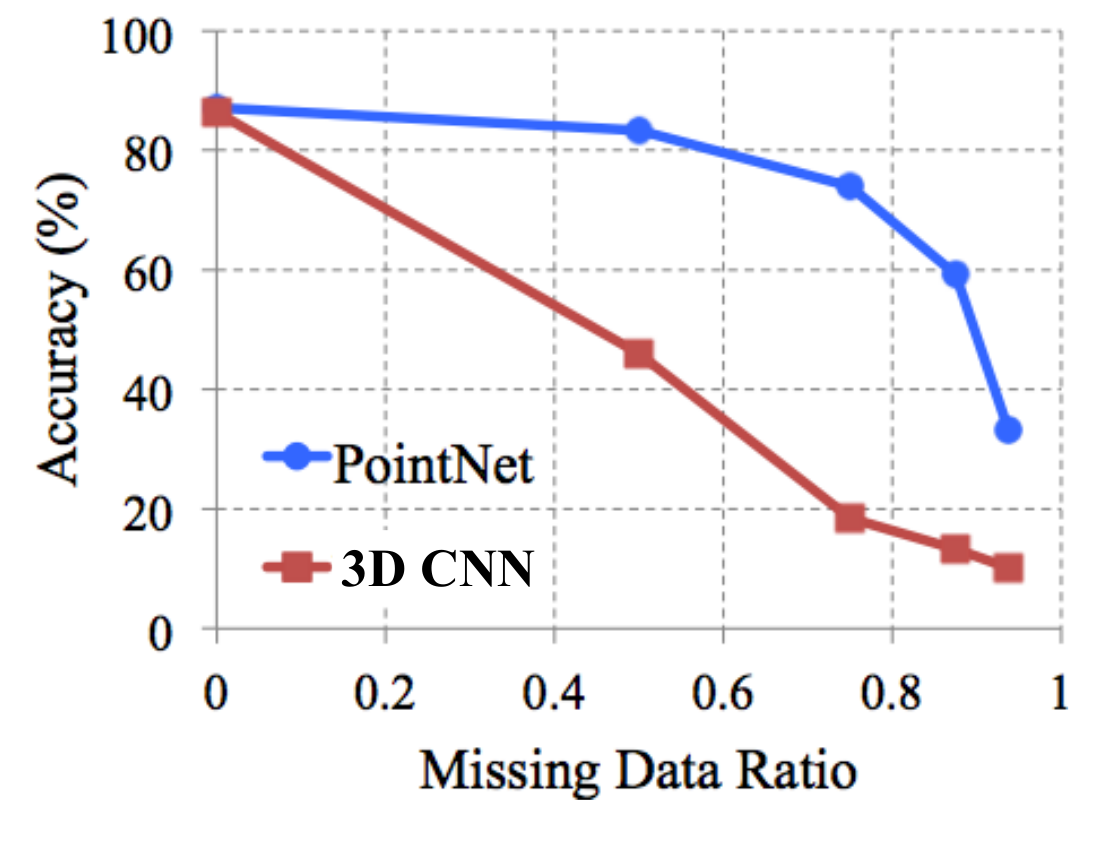
\includegraphics[height=0.7\textheight]{robustness_comp}
        \column{0.3\textwidth}
        Q: Why is PointNet so robust to missing data?
    \end{columns}
    \blfootnote{\textbf{Robustness in comparison with 3D CNN.} Figure from CVPR presentation to \cite{qi2017pointnet}.}
\end{frame}
